\chapter{TECNOLOGIAS EMPREGADAS}
\thispagestyle{empty}

Para o desenvolvimento do Atividades Complementares foi essencial o uso de algumas ferramentas as quais pudessem ser incorporadas  e tornassem possível a criação de funcionalidades para este projeto.

Ao longo de muitos anos, uma pergunta é feita por vários desenvolvedores. Qual o melhor Framework de desenvolvimento web já criado? Contudo esta é uma pergunta respondida de diversas formas, com base em vários argumentos e situações. E a resposta entretanto continua a mesma - Aquela que aumenta a produtividade e diminui esforços no  desenvolvimento. E depois de muito estudo e debate fora concluído que um Framework que reduza códigos gigantes e por muitas vezes difíceis de se ler e que sem margem de duvida diminuem o aprendizado são aqueles que aumentam a produtividade. Se buscarmos mais a fundo iremos nos debater com vários web Framework que focam em produzir aplicações, sejam elas web ou não. No entanto essas pecam em dois pontos vitais: produtividade e aprendizado. Um equilíbrio teve de ser estabelecido entre esses fatores e foi nesse momento que Ruby surgiu precedido do Rails como seu Framework de desenvolvimento web.

Serão apresentadas as seguintes tecnologias:
RVM como ambiente virtual para o desenvolvimento, Ruby como linguagem de programação, Rails como web framework, Mysql como base de dados inicial, MongoDB como base de dados conclusiva e o mais importante RubyGems para auxiliar na produção do sistema, git como ferramenta de repositório de código compartilhado com menbros do projeto.


\section{RVM (Ruby Version Manager)}

RVM é uma ferramenta de linha de comando que permite ao usário facilemte instalar, gerenciar e possuir varios ambiente de desenvolvimento ruby em uma só máquina com suas respectivas versões de rubygems.


\subsection{Ruby}
\label{Rvm}

Foi desenvolvida em 1994, e apresentada ao publico em 1995 por \textbf{Yukihiro Matsumoto}, que é mundialmente	conhecido como Matz que para criar ruby uniu partes das suas linguagens favoritas 
(\textit { Perl, Smalltalk, Eiffel, Ada, e Lisp }) para formar uma nova linguagem que equilibra a \textit{ programação funcional com a programação imperativa}. Passou a se tornar realmente reconhecida através de \textbf{ Dave Thomas }, mais conhecido como um dos \textit{“Programadores pragmáticos”}, que adotou o Ruby como uma de suas linguagens preferenciais e acabou escrevendo um dos livros mais completos sobre a linguagem, o Programming Ruby. Com isso	o número de adeptos a essa linguagem subiu muito rápido no ocidente. Ruby é uma das únicas linguagens nascidas fora do eixo EUA/Europa, sendo criada no Japão.

Matz criou uma linguagem mais poderosa que Perl e mais orientada a objetos que python. Em Ruby tudo é objeto, e possue métodos que podem ser facilemte acessados e modificados. O tornando assim uma linguagem mais simples de se ler e ser compreendida, facilitando o desenvolvimento e manutenção de sistemas escritos com com essa base. Um dos objetivos principais da linguagem é a praticidade. É possível que seja feito um algoritmo simples, sem precisar que se preocupe com as limitações da linguagem ou do interpretador.

O Ruby possui algumas características para manter a sua praticidade, como, uma linguagem enxuta que quase não há necessidade de colchetes e outros caracteres; a disponibilidade de diversos métodos de geração de código em tempo real, como os "attribute accessors";

\begin{center}
  \textit{"Ruby é simples na aparência, mas é muito mais complexo no interior, tal como o corpo-humano!"} - Ruby-Talk, \cite{MATZ}.
\end{center}


Uma forma prática de se instalar bibliotecas em ruby é através de \textbf{ \textit{ RubyGems } }, com ela é possível instalar e atualizar bibliotecas com uma única linha de comando, de maneira muito similar com os gerenciadores de pacotes de ambientes operacionais linux ou unix; Ruby possui uma notação muito utíl aos desenvolvedores, estas são chamadas de blocos de código, que ajudam o programador a passar um ou mais trechos de instruções para o método descrito em suas classes concretas. Ruby possui o contexto de Mixins, que simula herança múltipla, sem cair em seus respectivos problemas encontrados em outras linguagens. Ruby é classificado como dinamicamente tipado, por esse meio todos os tipos são objetos, não há tipos primitivos como era e ainda é feito em outras linguagens do genero como \textbf{ C++, Java(...) }, bem como suas definições de classes. No entanto variáveis de instância que por sua vez referenciam estes objetos não possuem um tipo específico. Um exemplo clássico em ruby seria uma reescrita da classe Fixnum nativa do ruby.
\\
\\
{\singlespace
\begin{lstlisting}[caption=Exemplo de uma \textit{Reescrita} de Classe,language=Ruby,label={test}]
[Irb]
[irb - prompt]
  2.1.0 :001 > class Fixnum
  2.1.0 :002 >  alias_method :old_add, :+
  2.1.0 :003 >  def plus(other)
  2.1.0 :004 >    self.old_add(other) * 2
  2.1.0 :005 >  end
  2.1.0 :006 > end

[irb - prompt]
  2.1.0 :007 > numero = 2 + 2
  2.1.0 :008 > numero
   "8"
  2.1.0 :009 > numero = nil
\end{lstlisting}
}

O operador \textit{plus} ou + é um método em Ruby, ao contrário de outras linguagens existentes. O resultado desse método reescrito na classe Fixnum diz que todoo e qualquer numero somado com o método soma, ira sempre executar a operação de soma em conjunto com o operador de multiplicação neste caso todo numero somado será multiplicado por dois após a operação anterior, e logo em seguida pelo fato de ruby ser dinamicamente tipado, o valor da variável \textbf{numero} é alterado para nil, o que siguinifica que podemos alterar o contexto de uma variável ou até mesmo inserção de código em tempo de execução.

Ruby possui uma ferramenta muito interessante, semelhante ao array visto em outras linguagens o ruby hashes, bastante similar ao dicionario de dados do python. Um ruby hashe utiliza chaves em vez de colchetes precedido de literais. O literal deve fornecer: uma chave e um valor agregados.
Por exemplo, se quiséssemos mapear os dados de um usuário poderíamos faze-lo da seguinte forma:

{\singlespace
\begin{lstlisting}[caption=Exemplo de um \textit{Ruby Hash},language=Ruby,label={ruby-hash}]
    user_section = {
      name: 'xpto' ,
      email: 'xpto@xpto.com' ,
      password: 'headwind' ,
      nickname: 'headwind' ,
      prefered_language: 'Ruby On Rails with MongoDB'
    }
\end{lstlisting}
}

O conceito acima é muito semelhante a forma como o MongoDB manipula seus documentos um contexto que será explicado mais a frente.
\\

Ultimamente a linguagem tem sido foco da mídia especializada devido ao seu web framework feito em Ruby, o Rails desenvolvido por \cite{DAVIDHANSSON}. Ainda hoje, toda a responsabilidade, quanto a, implementações de novas funcionalidades, é do Matz. Todas as decisões relacionadas à linguagem tem que passar por ele antes de serem implementadas e virem à publico. E mesmo assim a comunidade Ruby é forte o suficiente pra sobreviver caso alguma coisa aconteça com o Matz. Pois  há muitas pessoas que estão conectadas ao código tanto quanto o próprio Matz. Uma das grandes diferenças das outras tecnologias open-source, é que não tem uma empresa bancando os seus custos. O projeto sobrevive de doações feitas pelos usuários satisfeitos e por empresas que conseguiram aumentar sua produtividade e performance usando apenas Ruby ou Ruby On Rails. Em uma de suas declarações Matz fala sobre o que ele esperava obter quando criou a linguagem:

"Eu conhecia muitas linguagens antes de criar o Ruby, mas nunca estava satisfeito com elas. Elas eram feias, rigorósas, mais complexas ou mais simples do que eu esperava. Eu queria criar a minha própria linguagem que me satisfizesse como programador. Eu sabia muito sobre o público a ser alcançado: eu mesmo. Para minha surpresa, muitos programadores do mundo todo sentiam o mesmo que eu. Eles ficaram felizes quando descobriram e programaram no Ruby. Do começo ao fim do desenvolvimento da linguagem Ruby, concentrei minhas energias para fazer uma programação rápida e fácil. Todas as características do Ruby, incluindo as características de orientação a objetos, são designadas a funcionar com programadores comuns (por exemplo: eu) que esperam que elas funcionem. A maior parte dos programadores acha que ele é elegante, fácil de usar e sentem prazer em usá-lo."\cite{MATZ}.

\subsection{RubyGems}
\label{Ruby}

Uma RubyGem ou simplesmente \textit{Gem} é uma biblioteca como em qualquer outra linguagem de programação já criada, por exemplo: \textbf{ Python, Java, C++, C }, especificas  para  Ruby, que fornecem um formato padrão para aplicações. Uma Gem é escrita especialmente para facilitar o uso de determinada funcionalidade. Uma Gem é um conjunto de arquivos feitos em Ruby, etiquetados com nome e versão, cada uma possui, em seu escopo todas as características correspondente a sua arquitetura via um arquivo de configuração chamado \textbf{"gemspec"}. Tomando como exemplo a gem 'rspec-rails' que possui em seu escopo  arquivo rspec-rails.gemspec que possui toda a especificação desta desde qual o grupo responsável por mante-la com atualizações constantes, licenças e dependências. Gems podem ser utilizadas para estender ou modificar certas funcionalidades, geralmente são distribuídas por outros desenvolvedores Ruby mais conhecidos como \textbf{ \textit{ rubistas } }, varías delas possuem até mesmo comandos expecificos auxiliar e agilizar o desenvolvimento, além de que em Ruby rubygems podem ser integradas umas com as outras para facilitar ainda mais os ruby programadores.

\subsection{Como Ruby carrega RubyGems}
\label{Ruby}

Antes de tudo é  muito útil saber como o Ruby carrega arquivos de dependência. O Ruby seja na verão 1.9.3 ou mais recente predispõem de um comando bem simples o require "arquivo" com ele é possível carregar arquivo(s) diretamente ou especificando o caminho absoluto. Contudo existe ainda uma outra forma pouco usada o load "arquivo.rb". A única diferença é que com load deve ser colocado a estenção do arquivo e além disso se ao tentar executar o require novamente essa operação será negada pois este carrega uma vez esse arquivo, já o load permite carregar varias vezes. Load é muito útil quando se está testando um arquivo que está sofrendo alterações constantes. Existe ainda uma outra forma de se carregar arquivos é o require File.expand\_path("./../spec\_helper")                                                                                                                                                                                                                                                                                                                                                                                                                                                                                                                                                                   

{\singlespace
\begin{lstlisting}[caption=Exemplo de require e load Ruby 1.9.3 - 2.1.0,language=Ruby,label={test}]
[Irb]
[irb - prompt - 1.9.3]
  1.9.3 :001 > require 'lib/fixnum'
    true
  1.9.3 :002 >

[irb - prompt - 1.9.3 - Full-Path]
  1.9.3 :001 > File.expand\_path("./../spec_helper")
    true
  1.9.3 :002 >

[irb - prompt - 2.1.0]
  2.1.0 :001 > load 'lib/fixnum.rb'
    true
  2.1.0 :002 >
\end{lstlisting}
}

Como pode ser visto o comando  require pode carregar arquivos usando caminhos relativos. Porém também pode ser usado caminhos absolutos. Para tal quando se deseja carregar alguma dependência em um projeto Ruby existe um arquivo chamado \textbf{"rubygems.rb"} localizado em \textbf{~/.rvm/rubies/ruby-2.1.0/lib/ruby/2.1.0} ao qual contem toda a
expecificação de Gems como carregalás na versão decorrente do ruby instalado. Logo se precisa carregar esse arquivo toda vez que se deseja utilizar alguma gem:

{\singlespace
\begin{lstlisting}[caption=Exemplo de require 'rubygems',language=Ruby,label={require}]
  require 'rubygems'
  require 'BCrypt'
\end{lstlisting}
}

\subsection{Versionamento de Gems}
Versionamento é considerado por muitos a parte mais importante das RubyGems. É possível ter diversas versões na mesma máquina carregadas em
paralelo, essa é considerada a parte mais vantajosa e a principal fonte de confusão. Por exemplo: ao utilizar o comando 'gem list --local' 
uma lista será retornada contendo todas as Gems instaladas no momento. Essa lista pode e deve variar de máquina para máquina de acordo com 
as gems instaladas, para exemplificar  esse conceito seria como descrito na saída do terminal a seguir:

{\singlespace
\begin{lstlisting}[caption=Exemplo de versionamento de gems,language=Ruby,label={versionamento}]
  >> mongoid ( 3.0.0, 4.1.0)
\end{lstlisting}
}

Nesse trecho se carregarmos essa Gem uma mensagem de erro seria exibida, devido ao nome da Gem que não é o nome que o comando 'require' precisa, bem como a versão que se deseja carregar.
No entanto como fazer para carregar essa gem se o nome da mesma e o arquivo Ruby diferem nesse contexto? 

"Quando a convenção falha precisamos dizer explicitamente o que queremos."\cite{AKITA}.

{\singlespace
\begin{lstlisting}[caption=Exemplo de versionamento de gems,language=Ruby,label={versionamento}]
  >> require 'rubygems'
  >> gem 'mongoid'
  >> require 'mongoid'
\end{lstlisting}
}

O que foi feito no trecho anterior resolve o problema de nomes e carrega a versão mais atual da gem 'mongoid', caso a gem requerida seja 
uma versão que difere da atual, o desenvolvedor deverá especificar qual a versão da gem propriamente dita quer utilizar:


{\singlespace
\begin{lstlisting}[caption=Exemplo de versionamento de gems,language=Ruby,label={versionamento}]
  require 'rubygems'
  gem 'mongoid', '~> 3.0.0'
  require 'mongoid'
\end{lstlisting}
}

\section{Organização de aplicações web}

Construir aplicações web em Ruby on Rails é um pouco mais profundo do que simplesmente construir páginas atras de páginas como era feito antigamente.
A razão para tudo isto é que ele é preparado para atender e criar aplicações modernas e arrojadas(sofisticadas) e isto quer dizer que a aplicação desenvolvida
sobre esta plataforma não deve apenas responder por páginas HTML mas de forma adequada e dinâmica em aplicações ricas em client-side em conjunto com outros 
frameworks como backbone.js entre outros.

\subsection{Aplicações ricas em client-side}
Antes de pensarmos em client-side deve-se ter em mente um conceito de aplicações web. Olhando o modelo server-side - MVC tradicional - Model, View e Controller, 
sendo todos executados no lado do servidor, gerando todo o html em conjunto com suas respectivas actions(requisições), para serem visualizadas pelo usuário em um web-browser

\begin{figure}[ht]
    \centering
    \scalebox{0.4}{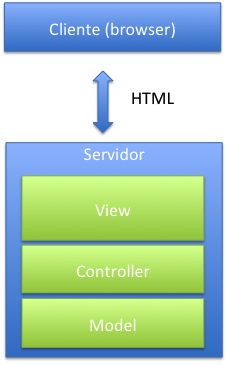
\includegraphics{figuras/server_side_mvc}}
    \caption{Modelo MVC básico}
    \label{submeter}
\end{figure}

Foi se criado um formato um pouco mais rebuscado, mais evoluido e nesse formato tem-se aplicações onde o html é gerado no lado do servidor, mas foi criada uma técnica conhecida
por muitos como ajax, para atualizar partes de páginas ou até mesmo funcionalidades implementadas para melhorar o desempenho do usuário evitando um reload completos
da página a cada iteração. Contudo ainda neste ponto parte do MVC é executado no lado do servidor e apenas a parte das Views são executadas no lado do cliente. Este modo eram
chamado de hibrido por muitos.

\begin{figure}[ht]
    \centering
    \scalebox{0.4}{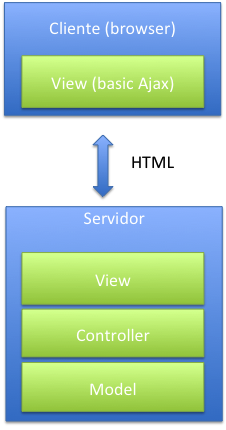
\includegraphics{figuras/hibrid_mode_mvc}}
    \caption{Modelo MVC hibrido}
    \label{submeter}
\end{figure}

Depois de muito se estudar o conceito de modelo MVC - Standard e MVC - hybrid um terceiro modelo surgiu e é nesse que as aplicações client-side executam atualmente e neste a arquitetura
MVC é toda executada em client-side (Lado do clientte ). O Model passa ter entretanto duas atribuições de responsabilidade, a de fornecer toda a API bem como as validações executadas no
lado do servidor, e outra que é executada no lado do cliente que também oferece validações sobre a estrutura do modelo exibido.
\\\\\\
\begin{figure}[ht]
    \centering
    \scalebox{0.4}{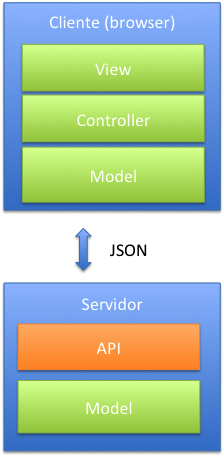
\includegraphics{figuras/client_side_mvc}}
    \caption{Modelo MVC Client-Side}
    \label{submeter}
\end{figure}

Em resumo o Modelo MVC pode ser descrito como uma série de requisições solicitadas pelo Browser e interpretadas pelo servidor que possui uma via
de mão dupla.

\begin{figure}[ht]
    \centering
    \scalebox{0.4}{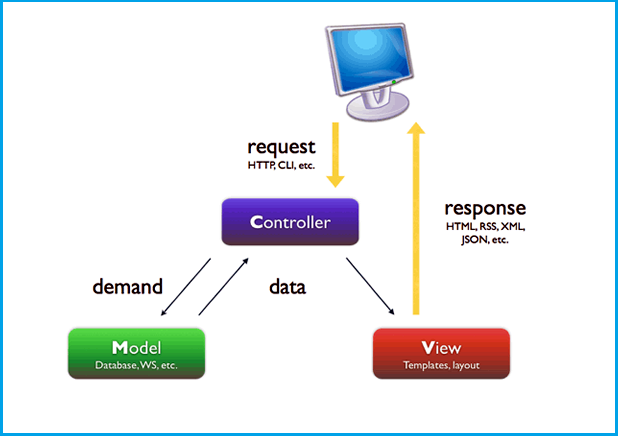
\includegraphics{figuras/mvc_complete}}
    \caption{Modelo MVC}
    \label{submeter}
\end{figure}


Desenvolver aplicações voltadas para client-side possuem algumas vantagens importantes como:
\begin{itemize}
    \item{ \textbf{Melhor desempenho para o usuário:}
      sendo esta uma das principais vantagens no que diz respeito ao desempenho de cada browser, não ter que precisar 
      fazer requisições a todo momento, na hora de fazer dowload, ou atualizar a página completa a cada iteração do 
      usuario com esta. Aplicações feitas em client-side funcionam tao bem quanto aplicações feitas para desktop.
    }
    \item{ \textbf{Melhor desempenho na transferência de dados:}
      Há também um ganho considerável na taxa de transmissão dos dados, ao invés de carregar o cenário da página html completa
      a cada interação do usuário, na arquitetura client-side todo o cenário é transferido na primeira solitação e as requisições 
      seguintes são responsáveis por trafegar apenas os dados consolidados entre o cliente e o servidor, normalmente no formato JSON. 
    }
    
    \item{ \textbf{Facilidade de manutenção:}
      com aplicações em client-side a API forncecida pelo servidor possibilita a facilidade de manutenção de forma independente ao usuário,
      de tal forma que o cliente não perceberá quando a página sofrer atualizações em tempo não real.
    }
    
    \item{ \textbf{Redução de carga no lado do Servidor:}
      O sistema completo passa a ser enviado ao usuário final através de arquivos html, css e javascript que podem ser comprimidos 
      e distribuídos através de CDN's com faclidade. Uma vez baixados esses arquivos são mantidos em cache no browser da preferência do usuário. 
      O servidor tem a responsabilidade apenas de fornecer uma API, enviar e receber os dados no formato JSON. Dessa forma todo o processamento 
      é responsável por particionar dos dados e  a geração de templates fica exclusivamente no lado cliente e não mais no servidor, liberando recursos. 
    }
\end{itemize}

\section{Ruby On rails}

RoR é um web framework escrito sob a linguagem Ruby. Criado por \cite{DAVIDHANSSON} em 2003, baseado em seu trabalho no Basecamp, que é 
uma ferramenta de gerenciamento de projetos 37 signals. No entanto David só lançou o RoR como código aberto em julho de 2004, e mais tarde em dezembro de 
2005 foi lançada a primeira versão do Ruby on Rails.

Assim como outros frameworks de aplicação web o RoR utiliza a arquitetura  MVC(model view controller), fornecendo um isolamento entre a lógica de negócio 
dos modelos, a interface com o usuário através das views e a manipulação de todas as requisições no servidor de apicação. O que contribui muito para que a manutenção do código seja bem mais fácil e flexível.

Ruby on Rails possui uma filosofia que segue dois princípios:
\begin{itemize}
 \item {DRY}
 \item {CoC}
\end{itemize}

\subsection{DRY}
Don't Repeat Yourself(Não se repita). Se aplicado corretamente, possibilita a reduzir a duplicação de tarefas dentro de um projeto. Réplicas ou duplicatas de qualquer
tipo, dentro de uma aplicação, leva a dificuldade de modificação e manutenção e inconsistência, sem levar em conta em alguns casos a ilegibilidade do source-code. 
Em RoR, se pode ver este princípio em ação em quase tudo, desde as componentes reutilizáveis em forma de plug-ins para a forma como as tabelas da base de dados escolhida são mapeadas.

\subsection{CoC}

\textit{Convenção sobre Configuração} ou \textit{programação por convenção} vem do termo em inglês \textbf{(Convention over Configuration - CoC)}, uma prática de desenvolvimento de software que visa diminuir o nnumero obsoleto de decisões que os desenvolvedores precisam tomar ao longo de seus projetos. Estabelecendo simplicidade sem preder flexibilidade.
Quando um desenvolvedor seja ele experiente ou não for iniciar atividades em Rails, o usuário estará sempre na maior parte do tempo interagindo com os controllers, views e models entre outras palavras a arquitetura MVC amplamente vista em design patterns e além desse fator importante estara diretamente conectato para a base de dados escolhida seja ela 
relacional ou não relacional como no caso dos NoSQL. De tal forma a reduzir a necessidade de configuração pesada.

RoR permite a criação de regras personlizadas, contudo é sempre  uma boa idéia usar as convenções que o própio	Rails oferece, essas convenções deverão acelerar o desenvolvimento, manter um código limpo, conciso e legível e o mais importante estas convenções permitem uma navegação muito mais fácil dentro da aplicação.
Rails não foi baseado  em um único padrão de desenvolvimento, mas sim uma série de padrões. Outros frameworks que faziam parte do núcleo do Rails antigamente foram removidos desse núcleo afim de reduzir o acoplamento e com isso e permitir que quem o esteja utilizando os substituam sem  muita dificuldade, mas continuam funcionando e sendo usados em conjunto. Aqui estão alguns deles:

\subsection{Active Record}
Para se entender este item sendo este um dos mais importantes para se construir uma aplicação em Rails é necessário compreender um dos fundamentos mais criteriosos em orientação a objetos
o conceito de ORM(Object-Ralational Mapping) que pode ser traduzido como Mapeamento Objeto Relacional e segundo \cite{TECTARGET}, trata-se de uma forma rapida e prática de relacionar e endereçar, e manipular objetos sem que seja, necessário se preocupar com a forma ao qual estes se comunicam e se relacionam entre si.
ORM possibilita aos desenvolvedores experientes ou novatos à manter a uma perspectiva consistente dos objetos no percurso do projeto, mesmo que haja alteraçãoes no código ou até mesmo na base de dados em questão.

De acordo com \cite{BAKHARIA}, o \textbf{Active Record} cria uma abstração de \textit{OODB} - \\ (Orientação a Objeto em Banco de dados) onde o rails cria um mapeamento relacional entre tabelas e classes do modelo ao qual estas pertencem. Sendo que o Active Record também fornece uma série de métodos nas próprias classes para trabalhar com a manipulação de dados, como por exemplo criar, salvar, atualizar, deletar, entre outras palavras todas operações para gerenciar o CRUD do modelo descrito.
Ao contrário de outras bibliotecas complexas o Active Record não necessita de configurações desse nível, além de ser capaz de se dispor da capacidade de propor mapeamentos objeto relacional com base em convenções de nomenclatura de tabelas e nome dos campos o que ajuda a justificar a importância do conceito chave de desenvolvimento a idéia de \textit{ Convention Over Configuration(Convenção Preferível à Configuração) } o que a mesma afirma que com esse pretexto o Active record torna o Ruby On Rails uma das ferramentas de desenvolvimento web mais ágil para a produção de sistemas com banco de dados.

Na Prática todo e qualquer modelo criado pelo gerador de componentes do rails o mesmo estende a classe nativa \textbf{ActiveRecord::Base} responsável por abstrair uma entidade contida na base de dados, assim como cada objeto representa uma linha do banco de dados como menciona \cite{PRAGMATICRUBY}.

\subsection{Action Controller}
Segundo \cite{ORSINI}, em qualquer aplicação feita em rails, um controller é uma especialização da classe \textbf{Action Controller} que oferece uma série de conjunto de regras de negócio para a aplicação
Geralmente cada controller responde ao modelo ao qual encontra-se alocado, podendo este ser o que muitos chamam de \textbf{Controller Virtual}. Um Controller Virtual também é chamado de controller genérico, 
que não necessáriamente está associado à um modelo.

\subsection{Action View}
Segundo \cite{BAKHARIA}, Action View é um dos componentes responsável apenas por gerar a interação entre a aplicação e o usuário. Um Controller pode ter várias actions( métodos ), e para cada action dependendo da situação uma view para esta que automáticamente é reconhecida e exibida.
Um action view também é conhecida como template. Esse template pode reproduzir vários elementos, não só o html, mas também outros tipos como XML, JavaScript, PDF.
O template nada mais é do que uma renderização de código ruby com Html e possivelmente Javascript.


\subsection{Action Support}
"Active Support é composto por uma série de bibliotecas compartilhadas por todos os componentes gerenciados pelo Rails. 
Muito do que está acoplado nesse módulo está destinado a uso interno do Rails.
No entanto, Active Support também estende algumas das classes internas de Ruby de maneira útil e interessante."\cite{PRAGMATICRUBY}.

\subsection{Action Mailer}
ActionMailer é um componente nativo do rails que permite que a aplicação desenvolvida possa enviar correio-eletrônico. 
\\
"É importante um sistema que facilite a operação de envio de mensagens de e-mails porque
essa é uma operaão tem diversas aplicações comuns como: Enviar e -mails de confirmação de
cadastro; Notificações de erros ao administrador do site; Confirmação de compra de produtos
em lojas virtuais; Newsletters".\cite{BAKHARIA}
\\
\noindent A classe Mailer do Rails possui métodos para diferentes formas de enviar mensagens de acordo com o que a aplicação necessita. O formato de saida dessa mensagem
e descrito em sua ActionView de forma muito similar com as actions views gerenciadas pelos erb.

\subsection{Rake}

Rake é conhecido como Ruby Make, um utilitário autônomo Ruby que substitui o utilitário Unix 'make'
e usa um "Rakefile' e arquivos com extensão .rake para criar uma lista de tarefas. No Rails, Rake é
usado para tarefas comuns de administração, especialmente os mais sofisticados que constroem fora de si.
Pode-se obter uma lista de tarefas Rake disponíveis simplesmente digitando rake - tasks.
Cada tarefa tem uma descrição, o que deve ajudar a encontrar funções expecificas para o que se deseja

\subsection{Migrations}
O Migration pertime alterar o esquema de banco de dados ao longo do tempo de uma forma consistente e fácil.
Ele utiliza uma DSL do ruby para que nao tenha que escrever SQL a mão, fazendo assim com que as mudanças no banco de dados
seja independente. Cada migration é uma nova "versão" do banco de dados. Um esquema começa vazio e a cada migration ele é modificado
para acrescentar ou remover tabelas, colunas ou entradas necessárias.

\subsection{Organização de arquivos em Rails}
RoR se dispõe de ferramentas de desenvolvimento rápido e sem muito esforço. Para se iniciar uma nova aplicação em rails
bastaria usar o comando inicial:

{\singlespace
\begin{lstlisting}[caption=Exemplo de uso de scaffold, language=Ruby,label={scaffold}]
  >> rails new my_new_rails_app [ -d  ] { options }
\end{lstlisting}
}

Ao utilizar esse comando inicial toda uma estrutura de arquivos e diretórios é criada. 

\begin{figure}[ht]
    \centering
    \scalebox{0.4}{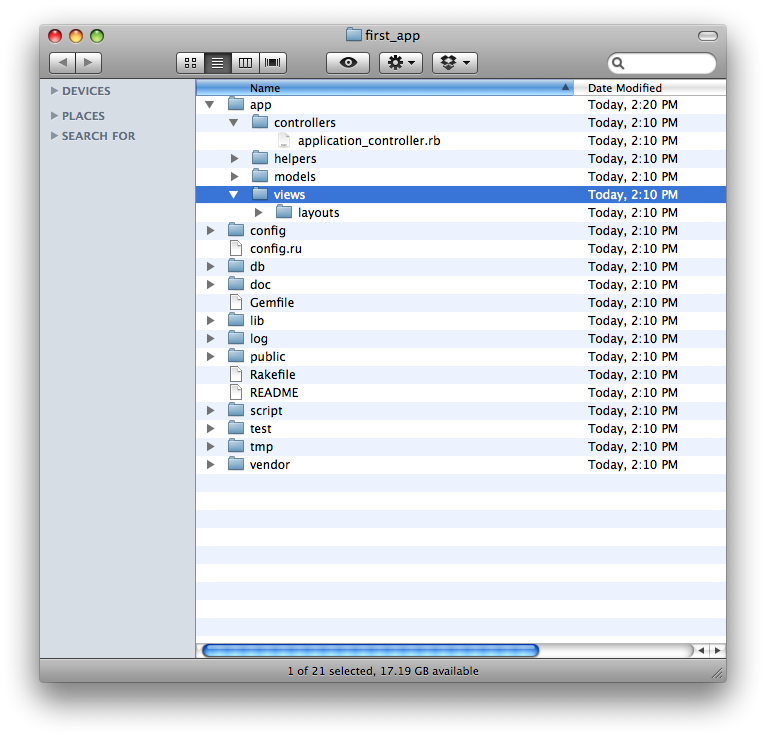
\includegraphics{figuras/rails_app}}
    \caption{Estrutura básica de arquivos e diretórios}
    \label{submeter}
\end{figure}

É possivél ainda passar parametros para a criação da mesma tais como:
o -d siguinifica qual a base de dados a ser utilizada, RoR possui três ambientes de integração: \textbf{development} responsável apenas pela etapa de desenvolvimento, 
este recarrega todas as classes sempre que uma nova action é requisitada, portanto uma nová cópia da classe é obtida, incluido qualquer alteração recente na mesma,
\textbf{test} - o próprio nome similar ao nosso português já indica que este é um ambiente onde se pode criar os testes contidos na aplicação que see tornarão a documentação
executavel da aplicação desenvolvida e por ultimo RoR possui um ambiente - \textbf{production} - onde o RoR carrega a classe apenas uma única vez, é onde a aplicação irá rodar em produção constante em um servidor de aplicação,
sem a necessidade de sofrer alterações como normalmente é feito em desenvolvimento. Ainda existe uma série de parametros que se pode passar para a criação de uma aplicação em rails uma delas é a opção de usar ou não o ActiveRecord
que é nativo do rails ao utilizar "\textbf{--skip-active-record}" o desenvolvedor está explicitamente dizendo ao rails para criar uma aplicação sem persistência à uma base de dados relacional, com isso é possivel escolher alguma das
base de dados NoSQL como por exemplo MongoDB, CouchDB, Cassandra etc.
\\
\\
\subsection{Scaffolding}
Rails possui uma ferramenta de desenvolvimento ágil conhecida como scaffold, e essa ferramenta possibilita a criação do Model de acordo com os parâmetros expecificados.
Este comando possibilita a criação de todo o CRUD, controller, model e views deste modelo dito no ato da criação. Em uma aplicação rails dependende do que se deseja e dependendo 
da não complexidade o scaffold se faz uma boa escolha e para utiliza-lo basta usar:

{\singlespace
\begin{lstlisting}[caption=Exemplo de uso de scaffold, language=Ruby,label={scaffold}]
  >> rails g scaffold user username:string address:string birth_date:date
\end{lstlisting}
}

Em uma aplicação rails é sempre bom fazer uso de CoC, e nessas convenções o rails tem uma nomenclatura no que diz respeito a \textbf{controllers e models}, toda vez que um controller é criado
este sempre estará no plurar, já o model correspondente irá sempre estar no singular. Isto quando for utilizado o comando scaffold que no ato irá gerar uma série de outros arquivos além do controller, 
do model e das views responsáveis por gerenciar o modelo descrito.
\\
\begin{figure}[ht]
    \centering
    \scalebox{0.4}{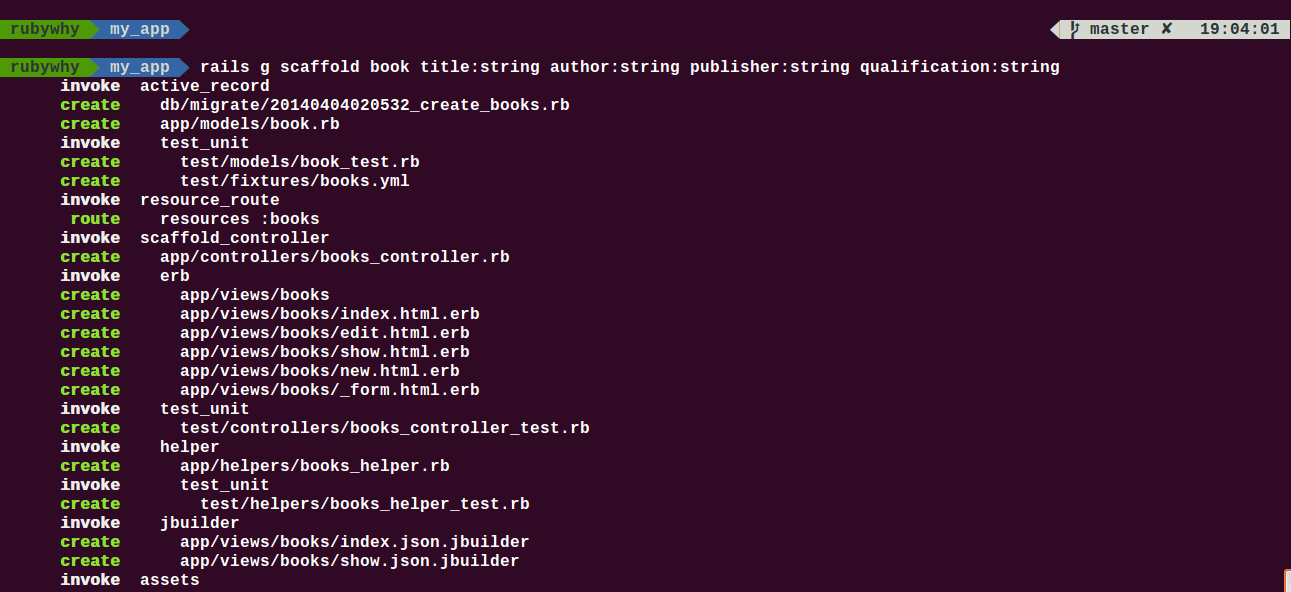
\includegraphics{figuras/scaffold_generator}}
    \caption{Parte dos arquivos criados após o scaffold.}
    \label{submeter}
\end{figure}
\\
A introdução deste comando \textit{rails g} possibilita ao desenvolvedor uma série de outros comandos
uma vez que pode ser abreviado, o nome por extenso para este comando é \textbf{generate}. O generate é o gerador de elementos do rails, com ele é possivel realizar outras 

\subsection{Comunidade Rails}

"A comunidade rubista/rails é hoje uma das mais ativas e unidas do Brasil. Cerca de 10 dos eventos que acontecem anualmente
ao redor do mundo com o único propósito de difundir conhecimento e unir os desenvolvedores. Um exemplo dessa força é o Ruby Conf, maior evento 
de Ruby da America Latina, com presença dos maiores nomes nacionais e internacionais de Ruby on Rails, e a presença de uma track dedicada ao 
Ruby na QCon São Paulo."\cite{CAELUM}.

\section{Git}
Git é um sistema de controle de versões distribuídas livre e de código aberto, projetado para lidar com qualquer projeto, desde o menor ao maior com rapidez e eficiência \cite{SOFTWARE-FREEDOM-CONSERVANCY}.

A historia do Git está muito relacionada a criação do Linux e de Linus Torvalds, seu criador, bem como com toda comunidade de desenvolvimento Linux. Durante anos a comunidade utilizou a ferramenta \textit{BitKeeper} para guardar a modificações do projeto.

Em 2005, após um problema com a proprietária deste, a comunidade decidiu criar sua própria ferramenta a partir da experiência com a anterior, houve um novo foco em: velocidade, \textit{design} simples, suporte para desenvolvimento paralelo, distribuição completa e a habilidade necessária para lidar com projetos grandes sem perda de velocidade e dados.

Assim, esse novo sistema de versionamento permite que qualquer repositório seja o centro do versionamento, deixando todo \textit{log} das modificações guardados nele sem que para isso precise de uma conexão a rede ou servidor geral.